\documentclass[twoside,twocolumn]{article}

\usepackage{blindtext} % Package to generate dummy text throughout this template 
\usepackage{graphicx}
\usepackage[sc]{mathpazo} % Use the Palatino font
\usepackage[T1]{fontenc} % Use 8-bit encoding that has 256 glyphs
\linespread{1.05} % Line spacing - Palatino needs more space between lines
\usepackage{microtype} % Slightly tweak font spacing for aesthetics

\usepackage[english]{babel} % Language hyphenation and typographical rules

\usepackage[hmarginratio=1:1,top=32mm,columnsep=20pt]{geometry} % Document margins
\usepackage[hang, small,labelfont=bf,up,textfont=it,up]{caption} % Custom captions under/above floats in tables or figures
\usepackage{booktabs} % Horizontal rules in tables
\usepackage{graphicx}
\usepackage{lettrine} % The lettrine is the first enlarged letter at the beginning of the text

\usepackage{enumitem} % Customized lists
\setlist[itemize]{noitemsep} % Make itemize lists more compact

\usepackage{abstract} % Allows abstract customization
\renewcommand{\abstractnamefont}{\normalfont\bfseries} % Set the "Abstract" text to bold
\renewcommand{\abstracttextfont}{\normalfont\small\itshape} % Set the abstract itself to small italic text

\usepackage{titlesec} % Allows customization of titles

\titleformat{\section}[block]{\large\scshape\centering}{\thesection.}{1em}{} % Change the look of the section titles
\titleformat{\subsection}[block]{\large}{\thesubsection.}{1em}{} % Change the look of the section titles

\usepackage{fancyhdr} % Headers and footers
\pagestyle{fancy} % All pages have headers and footers
\fancyhead{} % Blank out the default header
\fancyfoot{} % Blank out the default footer
\fancyhead[C]{Comparativa de las metodologìas de elaboración de Datawarehouse vs metodologias de elaboración de Datalakes $\bullet$ Abril 2022 $\bullet$ } % Custom header text
\fancyfoot[RO,LE]{\thepage} % Custom footer text

\usepackage{titling} % Customizing the title section

\usepackage{hyperref} % For hyperlinks in the PDF

%----------------------------------------------------------------------------------------
%	TITLE SECTION
%----------------------------------------------------------------------------------------
\providecommand{\keywords}[1]{
  \small	
  \textbf{\textit{\quad \quad Keywords: }} #1}

\providecommand{\pclave}[1]{
  \small	
  \textbf{\textit{\quad \quad Palabras Clave: }} #1}

%Idiomas: \selectlanguage{english} \selectlanguage{spanish}

\begin{document}

\title{Trabajo Encargado 04:Comparativa de las metodologìas de elaboración de Datawarehouse vs metodologias de elaboración de Datalakes}

\begin{titlepage}
\begin{figure}[htb]
\begin{center}

\includegraphics[width=5cm]{imagenes/logo.png}
\end{center}    
\end{figure}
\vspace*{-0.25in}
\begin{center}
\large{UNIVERSIDAD PRIVADA DE TACNA}\\
\vspace*{-0.025in}
INGENIERIA DE SISTEMAS  \\	

\vspace*{0.5in}
\begin{large}
TITULO:\\
\end{large}

\vspace*{0.1in}
\begin{Large}
\textbf{ Comparativa de las metodologìas de elaboración de Datawarehouse vs metodologias de elaboración de Datalakes} \\
\end{Large}

\vspace*{0.3in}
\begin{Large}
\textbf{CURSO:} \\
\end{Large}

\vspace*{0.1in}
\begin{large}
Inteligencia de Negocios\\
\end{large}

\vspace*{0.3in}
\begin{Large}
\textbf{DOCENTE:} \\
\end{Large}

\vspace*{0.1in}
\begin{large}
 Ing. Patrick Cuadros Quiroga\\
\end{large}

\vspace*{0.2in}
\vspace*{0.1in}
\begin{large}

Integrantes: \\
\begin{flushleft}
Maldonado Cancapi, Carlos Alejandro\hfill(2018000660) \\
Huillca Aroni, Alfredo\hfill(2018060903)\\
Anahua Huayhua, Jenny Karen\hfill(2018062150)\\
Coloma Colquehuanca, Kiara\hfill(2018062218)\\

\end{flushleft}
\end{large}

\vspace*{0.1in}
\begin{large}
Tacna - Perú\\
2022
\end{large}
\end{center}
\end{titlepage}

\setlength{\droptitle}{-4\baselineskip} % Move the title up

\pretitle{\begin{center}\Huge\bfseries} % Article title formatting
\posttitle{\end{center}} % Article title closing formatting
\title{Comparativa de las metodologìas de elaboración de Datawarehouse vs metodologias de elaboración de Datalakes} % Article title

\date{\today} % Leave empty to omit a date                     
\renewcommand{\maketitlehookd}{%

}

%----------------------------------------------------------------------------------------



% Print the title
\maketitle

%----------------------------------------------------------------------------------------
%	ARTICLE CONTENTS
%----------------------------------------------------------------------------------------

\section{Resumen}
En este documento se estudian, analizan y comparan diversas metodologías y herramientas para el desarrollo de un Data Warehouse (DW) y metodologías de elaboración de Datalakes que permita la integración de información en caso, o no que dichos datos se encuentren en diferentes motores de bases de datos y/o provengan de diferentes fuentes de datos, esto, con el fin de convertir los datos en información pertinente y para que dichos datos cumplan con características como la calidad y exactitud, entre otras. Con la gran ventaja de que una vez el Data Warehouse esté desarrollado, se puedan ejecutar procesos de Business Intelligence (BI) para lograr que la información pueda ser usada para la toma de decisiones. 

%------------------------------------------------

\section{Abstract}

This document studies, analyzes and compares various methodologies and tools for the development of a Data Warehouse (DW) and methodologies for the elaboration of Datalakes that allow the integration of information in case, or not, that said data is found in different database engines. of data and/or come from different data sources, this, in order to convert the data into relevant information and so that said data meets characteristics such as quality and accuracy, among others. With the great advantage that once the Data Warehouse is developed, Business Intelligence (BI) processes can be executed so that the information can be used for decision making. 



%------------------------------------------------
\section{Introduccion}

\begin{center}

\end{center}

\section{Desarrollo}

\subsection{DATA WAREHOUSE}

W.H. Inmon, considerado el padre de las bodegas de datos en el 92, define los Data Warehouse como: "Un sistema orientado al usuario final, integrado, con variaciones de tiempo y sobre todo una colección de datos como soporte al proceso de toma de decisiones". Por otra parte, Ralph Kimball, considerado como uno de los más importantes precursores y padre del concepto Data Warehouse, lo define como: "una copia de los datos de la transacción estructurados específicamente para preguntar y divulgar" . 

En la actualidad, con el fin de lograr un mejor rendimiento las organizaciones tienden a gastar su esfuerzo en la maximización de ingresos y minimizar los gastos, para conseguir dicha meta se requieren elementos que deben reflejarse desde los empleados de nivel más bajo hasta los altos mandos ejecutivos, esto se logra con unos arduos y tediosos procesos de análisis estratégicos para mejorar los procesos empresariales basados en las decisiones de quienes están al mando, es por esto que el lograr obtener informes consolidados o detallados de la información de la empresa, resulta vital en la toma de decisiones y es aquí donde entran en juego los DW, debido a que su propósito en simples cuentas es obtener informes detallados de la información de la empresa con el fin de mejorar la toma de decisiones 

\subsection{METODOLOGIAS}
\subsubsection{HEFESTO}
Con base en comprender cómo una organización puede crear inteligencia de negocios de sus datos, La metodología de Hefesto se divide en cinco fases y se sintetiza de la siguiente manera: 


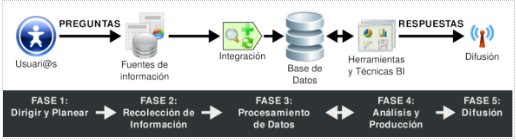
\includegraphics[width=7cm]{imagenes/img1.PNG}

\paragraph{- Fase 1: }

Dirigir y Planear.

En esta fase inicial es donde se deberán recolectar los requerimientos de información específicos de los diferentes 
usuarios, así como entender sus diversas necesidades, para que luego 
en conjunto con ellos se generen las preguntas que les ayudarán a 
alcanzar sus objetivos. 

\paragraph{- Fase 2:}
Recolección de Información.

Es aquí en donde se realiza el proceso de extraer desde las diferentes fuentes de información de la 
empresa, tanto internas como externas, los datos que serán necesarios 
para encontrar las respuestas a las preguntas planteadas en el paso 
anterior. 
\paragraph{- Fase 3:}
Procesamiento de Datos.

En esta fase es donde se integran y 
cargan los datos en crudo en un formato utilizable para el análisis. Esta 
actividad puede realizarse mediante la creación de una nueva base de 
datos, agregando datos a una base de datos ya existente o bien 
consolidando la información. 

\paragraph{- Fase 4:}
Análisis y Producción.

Ahora, se procederá a trabajar sobre 
los datos extraídos integrados, utilizando herramientas y técnicas propias 
de la tecnología BI, para crear inteligencia. Como resultado final de esta 
fase se obtendrán las respuestas a las preguntas, mediante la creación 
de reportes, indicadores de rendimiento, cuadros de mando, gráficos 
estadísticos, etc. 
\paragraph{- Fase 5:}
Difusión.

Finalmente, se les entregará a los usuarios que lo 
requieran las herramientas necesarias, que les permitirán explorar los 
datos de manera sencilla e intuitiva22 

\subsubsection{METODOLOGÍA DE RALPH KIMBALL }
La metodología de Kimball se basa en cuatro principios fundamentales: 
Centrarse en el negocio: Hay que concentrarse en la identificación de 
los requerimientos del negocio y su valor asociado, y usar estos 
esfuerzos para desarrollar relaciones sólidas con el negocio, agudizando 
el análisis del mismo y la competencia consultiva de los 
implementadores. 
Construir una infraestructura de información adecuada: Diseñar una 
base de información única, integrada, fácil de usar, de alto rendimiento 
donde se reflejará la amplia gama de requerimientos de negocio 
identificados en la empresa. 
Realizar entregas en incrementos significativos: crear el almacén de 
datos (DW) en incrementos entregables en plazos de 6 a 12 meses. Hay 
que usa el valor de negocio de cada elemento identificado para 
determinar el orden de aplicación de los incrementos. En esto la 
metodología se parece a las metodologías ágiles de construcción de 
software. 
Ofrecer la solución completa: proporcionar todos los elementos 
necesarios para entregar valor a los usuarios de negocios. Para 
comenzar, esto significa tener un almacén de datos sólido, bien diseñado, 
con calidad probada, y accesible. También se deberá entregar 
herramientas de consulta ad hoc, aplicaciones para informes y análisis 
avanzado, capacitación, soporte, sitio web y documentación. 
La construcción de una solución de DW es compleja, y Kimball propone una 
metodología que ayuda a simplificar dicha solución. Las tareas de esta 
metodología (ciclo de vida) se muestran en la siguiente figura:

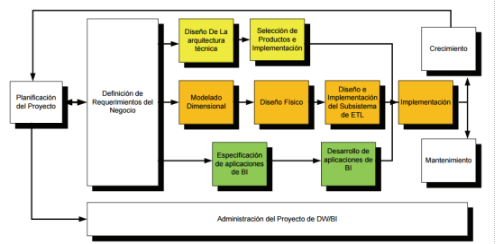
\includegraphics[width=6cm]{imagenes/img2.png}

\subsubsection{METODOLOGÍA CRISP-DM (Cross- Industry Standard PRocess for Data Mining). }
La metodología de CRISP es una de las principales metodologías por seguir por 
los analistas en la inteligencia de negocios, donde se puede rescatar 
primordialmente Data Warehouse y Data Mining. 
La metodología CRISP está sustentada en estándares internacionales que reflejas 
la robustez de sus procesos y que facilitan la unificación de sus fases en una 
estructura confiable y amigable para el usuario. Además de ello, esta tecnología 
interrelaciona las diferentes fases del proceso entre sí, de tal manera que se 
consolida un proceso iterativo y recíproco. Otro aspecto fundamental de esta 
tecnología es que es planteada como una metodología imparcial o “neutra 
respecto a la herramienta que se utilice para el desarrollo del proyecto de Data 
Warehouse o Data Mining siendo su distribución libre y gratuita. 
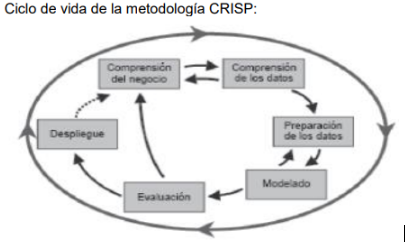
\includegraphics[width=7cm]{imagenes/img3.png}
El ciclo de vida del proyecto según la metodología según la metodología 
de CRISP está basado en seis fases cambiantes entre sí y nunca 
terminantes, lo cual lo postula como un ciclo en constante movimiento. 

\paragraph{- Comprensión del negocio:}
Se trata de entender claramente los 
requerimientos y objetivos del proyecto siempre desde una visión de 
negocio. Esta fase se subdivide a su vez en las siguientes categorías: 
o Definición de los objetivos del negocio (inicial, objetivos de 
negocio y criterios de éxito del negocio). 
o Evaluación de la situación (inventario de recursos, requisitos 
supuestos y requerimientos, riesgos y contingencias, terminología 
y costes y beneficios). 
o Definición de los objetivos del DW (objetivos y criterios de éxito). 
o Realización del plan del proyecto (plan del proyecto y valoración 
inicial de herramientas y técnicas). 

\paragraph{- Comprensión de los datos:}
Es conseguir y habituarse con los datos, 
reconocer las dificultades en la calidad de los datos y reconocer también 
las fortalezas de estos mismos que pueden servir en el proceso de 
análisis. Sus subdivisiones son: 

\begin{itemize}
    \item Recolección inicial de datos (informe de recolección). 
    \item Descubrimiento de los datos (informe descriptivo de los datos).
    \item Exploración de los datos (informe de exploración de los datos).
    \item Verificación de la calidad de los datos (informes de calidad). 
    
\end{itemize}

\paragraph{- Preparación de los datos:}
Es analizar los datos realmente importantes 
en el proceso de selección, depuración y transformación. Sus 
subdivisiones son: 
\begin{itemize}
    \item Selección de los datos (motivos para incluirlos o excluirlos). 
    \item Depuración de los datos (reporte de depuración).
    \item Estructuración de los datos (generación de atributos y registros)
    \item Integración de los datos (agrupar los datos).
    \item Formateo de datos (informe de la calidad de datos formateados).
\end{itemize}

\paragraph{- Modelado:}
Es la aplicación de técnicas de modelado o de Data 
Warehouse. Sus subdivisiones son: 

\begin{itemize}
    \item Selección de la técnica de modelado (técnica y sus supuestos). 
    \item Generar el plan de pruebas (plan de pruebas). 
    \item Construcción del modelo (parámetros escogidos, modelos, descripción de los modelos). 
    \item Evaluación del modelo (evaluar el modelo, revisión de los parámetro elegidos). 
\end{itemize}

\paragraph{- Evaluación:}
Esta fase es muy importante y decisiva, pues corresponde a 
la evaluación de la escogencia de los modelos anteriores y la toma de 
decisión respecto a si realmente son útiles en el proceso. Sus 
subdivisiones son: 
\begin{itemize}
    \item Evaluar resultados (valoración de los resultados respecto al éxito del negocio, modelos aprobados).
    \item Proceso de revisión (revisar el proceso).
    \item Determinación de los pasos siguientes (listado de posibles acciones, técnica modelada).  
\end{itemize}

\paragraph{- Despliegue o divulgación:}
Es la fase de implementación o de 
divulgación de los modelos anteriormente escogidos y evaluados. Sus 
subdivisiones son: 

\begin{itemize}
    \item Plan de divulgación o implementación (plan de implementación).
    \item Plan de monitoreo y mantenimiento (plan de monitoreo y mantenimiento).
    \item Presentación del informe fina (informe final, presentación final).
    \item Revisión del proyecto (documentación de la experiencia). 
\end{itemize}
\subsubsection{DWEP (Data Warehouse Engineering Process)}
Está basada en el proceso unificado 
estándar aceptado en el ámbito científico e industrial para el desarrollo de software; entre sus principales características se encuentra que es iterativo e incremental, se basa en cuatro fases de desarrollo y siete flujos de trabajo, en la Figura 3 se presentan gráficamente la relación existente entre los flujos de trabajo y las fases tanto del UP como de DWEP, está basado en componentes, utiliza el UML (Unified Modeling Language - Lenguaje Unificado de Modelado) como lenguaje para modelado gráfico es orientada a objetos, independiente de cualquier implementación específica, ya sea relacional o multidimensional y permite la representación de todas las etapas del diseño de un almacén de datos. 
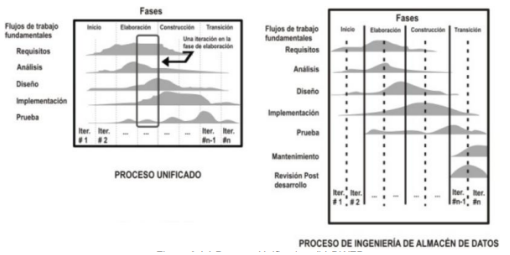
\includegraphics[width=7cm]{imagenes/img4.png}

\subsubsection{SEMMA}
Se define como el proceso de selección, exploración y modelado de grandes cantidades de datos para descubrir patrones de negocio desconocidos. Su nombre es el acrónimo correspondiente a las cinco fases básicas del proceso (muestro (sample), explotación (explore), modificación (modify), modelado (model), valoración (assess)) (28).  
\subsubsection{P3TQ (Product, Place, Price, Time, Quantity) }
Está compuesta por dos modelos, el Modelo de Negocio y el Modelo de Explotación de Información. El Modelo de Negocio proporciona una guía de pasos para identificar un problema de negocio o la oportunidad del mismo. El Modelo de Explotación de Información proporciona una guía de pasos para la ejecución de los modelos de explotación de información de acuerdo al modelo identificado en Modelo del Negocio.  
\subsubsection{KM-IRIS}
Fue elaborado por el grupo de Integración y Re-Ingeniería de Sistemas (IRIS) de la Universidad Jaume. Se crea con el objetivo de dirigir el proyecto de desarrollo de un sistema de gestión del conocimiento, consta de cinco fases: identificar, extraer, procesar, almacenar y compartir. Esta metodología pretende cubrir el ciclo completo en el desarrollo de un sistema de gestión del conocimiento. Es una metodología poco difundida y con escasa documentación (16, 27). En la tabla 1 se muestra una breve descripción de sus fases.
\subsubsection{Rapid Warehousing Methodology}
Es una metodología iterativa que está basada en el desarrollo incremental de un almacén de datos dividido en cinco fases. Esta metodología no incluye lo relativo a técnicas de análisis de la información, por lo que con su aplicación solo se obtendría el almacén de datos y no los multianálisis de los datos para apoyar la toma de decisión. 


\subsection{DATA LAKE}
Es un repositorio de almacenamiento que contiene una gran cantidad de datos en bruto y que se mantienen allí hasta que sea necesario. Se trata de guardar los datos con el objeto de que puedan ser procesados y utilizados en el momento en que sea necesario. Cada elemento del Data Lake recibe un identificador y etiquetas de metadatos extendidas, con el fin de que 20 pueda ser identificado y recuperado fácilmente. (Fang, 2015) Así, en el Data Lake pueden tener cabida muchos tipos de datos distintos, de diversas fuentes y en diferentes formatos. Esto exige, por supuesto, que la capacidad de almacenamiento sea enorme. En resumen, un sistema Data Lake permite retener todos los datos in procesamiento, dar soporte para todo tipo de perfiles de usuarios, tanto para modelos empresariales como científicos, de esta manera el acceso a la información original es más directa y reduce los pasos necesarios para su procesamiento, con una estructura de datos no definida hasta que los datos no son necesarios. 

\paragraph{Enfoque ágil:}
En un enfoque ágil es requerido para el diseño e implementación de data lake (Data Kitchen, 
2020) según data Kitchen, dado que se afrontan las siguientes dificultades: 

\begin{itemize}
    \item Demasiado trabajo
    \item Errores de datos
    \item Mala data arruina buenos reportes
    \item Cambios constantes de necesidades de negocio 
    \item Multitud de herramientas
    \item Mantenimiento de tuberia de datos nunca termina
    \item Fatiga de procesamiento manual
    \item Tareas desalentadoras en migración a nube
\end{itemize}

En la ejecución de proyectos de analítica de datos, se consideran tanto el ciclo de vida de los 
datos como el ciclo de vida de valor de negocio, partiendo de implementar una solución, pero 
afrontar el continuo cambio, como se observa en la siguiente tabla:
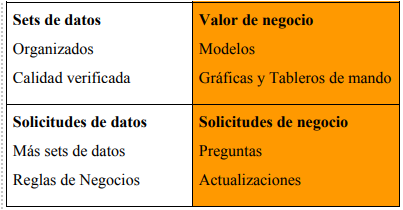
\includegraphics[width=7cm]{imagenes/img5.png}
Lo cual requiere que enfoques ágiles sean tenidos en cuenta, en cuanto a metodología, 
procesos y herramientas, considerando: 

\begin{itemize}
    \item Capacidad de realizar despliegues hacia ambientes de producción de manera rápida y segura. 
    \item Responder rápidamente a las solicitudes de integración de datos.
    \item Responder a los cambios de lógica de negocio.
    \item Tomar acciones correctivas sobre errores en datos oportunamente.
    \item Automatización de procesamiento y calidad.
    \item No quedar bloqueado en un enfoque centrado en herramientas o por restricciones de operación de herramientas.  
\end{itemize}


\section{Conclusiones}
Los lineamientos de diseño son la parte más importante de un proceso para el desarrollo de un DW, con esto bien especificado, el DW difícilmente falle en su funcionamiento y usando el esquema constelación, se tendrá una bonificación a nivel organizativo debido a su cualidad de ser específico. 

\section{Recomendaciones}
Se recomienda tener en cuenta que no todas las herramientas y metodologías no fueron estudiadas y comparadas, existen más de estas para ser analizadas y algunas pueden cumplir mejor para el desarrollo de un DW que las mencionadas en este documento.
Una vez se haya desarrollado un DW usando estas comparaciones, ya se podrán aplicar los procesos de BI que normalmente se aplican. 
 
 


%----------------------------------------------------------------------------------------
%	REFERENCE LIST
%----------------------------------------------------------------------------------------
\begin{thebibliography}{}

    \bibitem{DOC2008} 
    Data Lake vs Data Warehouse. Veamos sus principales diferencias. (2022). Powerdata.es. https://blog.powerdata.es/el-valor-de-la-gestion-de-datos/data-lake-vs-data-warehouse.-veamos-sus-principales-diferencias
    \bibitem{FRE2016} 
   Gorini, M. (2022). ¿Cuál es la diferencia entre un data lake y un data warehouse? Bismart.com. http://blog.bismart.com/diferencia-entre-data-lake-y-data-warehouse
	\bibitem{FRE2016} 
   Gigliotti, M. (2019). Data Lake y Data Warehouse: ¿Qué son y en qué se diferencian? Techedgegroup.com. https://www.techedgegroup.com/es/blog/data-lake-data-warehouse-definicion-diferencias
    \bibitem{FRE2019} 
   Data Lake vs Data Warehouse: Key Differences - Talend. (2022). Talend - a Leader in Data Integration Data Integrity. https://www.talend.com/resources/data-lake-vs-data-warehouse/
  
    \bibitem{FRE2019}
    Emilio Fernández Lastra. (2018, October 10). Data Warehouse y Data Lake. Qué son y para qué sirven. Artyco | the Data Driven Company. https://artyco.com/data-warehouse-data-lake-que-es/
    
    \bibitem{FRE2018}
   Prakash, S. S. (2020, April). Evolution of Data Warehouses to Data Lakes for Enterprise Business Intelligence. ResearchGate; unknown. https://www.researchgate.net/publication/343219651EvolutionofDataWarehousestoDataLakesforEnterpriseBusinessIntelligence/link/5f1d52ad92851cd5fa48958a/download
   
   \bibitem{FRE2018}
  Flores, A. (n.d.). Construyendo y governando Data Lakes y Data Warehouses modernos en AWS. Retrieved April 5, 2022, from https://d1.awsstatic.com/events/Summits/AMER2019/Mexico-City/BuildingandgoverningmoderndatalakesanddatawarehousesADB201.pdf
   
   \bibitem{FRE2018}
   Mendez, A., Britos, A.,  Garcia-Martínez, P. Y. (2003). Fundamentos de Data Warehouse. Reportes Técnicos En Ingeniería Del Software, 5(1), 19–26. http://artemisa.unicauca.edu.co/~ecaldon/docs/bd/fundamentosdedatawarehouse.pdf
    
    \bibitem{FRE2018}
    Agudelo, J. (2020) Data Lakes: Aplicaciones, Herramientas y Arquitecturas. Monografía presentada como requisito para optar al Título de Ingeniero de Sistemas y Computación https://repositorio.utp.edu.co/server/api/core/bitstreams/5f56e572-d416-487e-a6d5-ec3a8e45da46/content
 
	\bibitem{FRE2018}
	Pegdwendé Sawadogo, Jérôme Darmont. On data lake architectures and metadata management. Journal of Intelligent Information Systems, Springer Verlag, 2021, 56 (1), pp.97-120. ff10.1007/s10844- 020-00608-7ff. ffhal-03114365f https://hal.archives-ouvertes.fr/hal-03114365/document


 
    \end{thebibliography}


%----------------------------------------------------------------------------------------

\end{document}